\documentclass[aspectratio=169,12pt,t]{beamer}
\usepackage{graphicx}
\setbeameroption{hide notes}
\setbeamertemplate{note page}[plain]
\usepackage{listings}

% header.tex: boring LaTeX/Beamer details + macros

% get rid of junk
\usetheme{default}
\beamertemplatenavigationsymbolsempty
\hypersetup{pdfpagemode=UseNone} % don't show bookmarks on initial view


% font
\usepackage{fontspec}
\setsansfont
  [ ExternalLocation = ../fonts/ ,
    UprightFont = *-regular ,
    BoldFont = *-bold ,
    ItalicFont = *-italic ,
    BoldItalicFont = *-bolditalic ]{texgyreheros}
\setbeamerfont{note page}{family*=pplx,size=\footnotesize} % Palatino for notes
% "TeX Gyre Heros can be used as a replacement for Helvetica"
% I've placed them in fonts/; alternatively you can install them
% permanently on your system as follows:
%     Download http://www.gust.org.pl/projects/e-foundry/tex-gyre/heros/qhv2.004otf.zip
%     In Unix, unzip it into ~/.fonts
%     In Mac, unzip it, double-click the .otf files, and install using "FontBook"

% named colors
\definecolor{offwhite}{RGB}{255,250,240}
\definecolor{gray}{RGB}{155,155,155}
\definecolor{purple}{RGB}{177,13,201}
\definecolor{green}{RGB}{46,204,64}

\definecolor{background}{RGB}{255,255,255}
\definecolor{foreground}{RGB}{24,24,24}
\definecolor{title}{RGB}{27,94,134}
\definecolor{subtitle}{RGB}{22,175,124}
\definecolor{hilit}{RGB}{122,0,128}
\definecolor{vhilit}{RGB}{255,0,128}
\definecolor{codehilit}{RGB}{255,0,128}
\definecolor{lolit}{RGB}{95,95,95}
\definecolor{myyellow}{rgb}{1,1,0.7}
\definecolor{nhilit}{RGB}{128,0,128}  % hilit color in notes
\definecolor{nvhilit}{RGB}{255,0,128} % vhilit for notes

\newcommand{\hilit}{\color{hilit}}
\newcommand{\vhilit}{\color{vhilit}}
\newcommand{\nhilit}{\color{nhilit}}
\newcommand{\nvhilit}{\color{nvhilit}}
\newcommand{\lolit}{\color{lolit}}

% use those colors
\setbeamercolor{titlelike}{fg=title}
\setbeamercolor{subtitle}{fg=subtitle}
\setbeamercolor{institute}{fg=lolit}
\setbeamercolor{normal text}{fg=foreground,bg=background}
\setbeamercolor{item}{fg=foreground} % color of bullets
\setbeamercolor{subitem}{fg=lolit}
\setbeamercolor{itemize/enumerate subbody}{fg=lolit}
\setbeamertemplate{itemize subitem}{{\textendash}}
\setbeamerfont{itemize/enumerate subbody}{size=\footnotesize}
\setbeamerfont{itemize/enumerate subitem}{size=\footnotesize}

% page number
\setbeamertemplate{footline}{%
    \raisebox{5pt}{\makebox[\paperwidth]{\hfill\makebox[20pt]{\lolit
          \scriptsize\insertframenumber}}}\hspace*{5pt}}

% add a bit of space at the top of the notes page
\addtobeamertemplate{note page}{\setlength{\parskip}{12pt}}

% default link color
\hypersetup{colorlinks, urlcolor={hilit}}

\lstset{language=bash,
        basicstyle=\ttfamily\scriptsize,
        frame=single,
        commentstyle=,
        backgroundcolor=\color{offwhite},
        showspaces=false,
        showstringspaces=false
        }


% a few macros
\newcommand{\bi}{\begin{itemize}}
\newcommand{\bbi}{\vspace{24pt} \begin{itemize} \itemsep8pt}
\newcommand{\ei}{\end{itemize}}
\newcommand{\be}{\begin{enumerate}}
\newcommand{\bbe}{\vspace{24pt} \begin{enumerate} \itemsep8pt}
\newcommand{\ee}{\end{enumerate}}
\newcommand{\ig}{\includegraphics}
\newcommand{\subt}[1]{{\footnotesize \color{subtitle} {#1}}}
\newcommand{\ttsm}{\tt \small}
\newcommand{\ttfn}{\tt \footnotesize}
\newcommand{\figh}[2]{\centerline{\includegraphics[height=#2\textheight]{#1}}}
\newcommand{\figw}[2]{\centerline{\includegraphics[width=#2\textwidth]{#1}}}


%%%%%%%%%%%%%%%%%%%%%%%%%%%%%%%%%%%%%%%%%%%%%%%%%%%%%%%%%%%%%%%%%%%%%%
% end of header
%%%%%%%%%%%%%%%%%%%%%%%%%%%%%%%%%%%%%%%%%%%%%%%%%%%%%%%%%%%%%%%%%%%%%%

% title info
\title{Computer simulations}
\subtitle{The genomes of recombinant inbred lines}
\author{\href{https://kbroman.org}{Karl Broman}}
\institute{Biostatistics \& Medical Informatics, UW{\textendash}Madison}
\date{\href{https://kbroman.org}{\tt \scriptsize \color{foreground} kbroman.org}
\\[-4pt]
\href{https://github.com/kbroman}{\tt \scriptsize \color{foreground} github.com/kbroman}
\\[-4pt]
\href{https://twitter.com/kwbroman}{\tt \scriptsize \color{foreground} @kwbroman}
\\[-4pt]
{\scriptsize Course web: \href{https://kbroman.org/AdvData}{\tt kbroman.org/AdvData}}
}


\begin{document}

% title slide
{
\setbeamertemplate{footline}{} % no page number here
\frame{
  \titlepage

\note{
   This is a second case study, whose central lesson concerns the
   value of computer simulation, but which also concerns sort of a
   deep dive into a crazy probability problem that started out as a
   computer simulation but turned into a combination of simulation,
   numeric calculations, and analytic derivations (partly through
   symbolic, computational algebra).
}

} }



\begin{frame}[c]{}

\vspace*{-1mm} \hspace*{-2mm}
\figw{Figs/inbredmice.jpg}{1.2}

\note{
  My own research is in genetics, and I focus large on mouse genetics.

  Mice have a lot of advantages for biomedical research. One advantage
  is that you can generate inbred lines. That is, by repeated
  brother-sister matings, you can create a line that is entirely
  homozygous.

  The mice in this picture are members of an inbred strain, and so all
  are genetically identical. And mice like humans have two copies of
  every chromosome (one from their father and one from their mother),
  and because of the inbreeding those two copies are identical. So if
  you take a male and female from this strain and mate them, you get
  the same thing back.

  Thus, the mice you work with today are the same as the mice you'll
  work two years from now. And you can completely eliminate genetic
  variation from your studies. Or you can introduce genetic variation
  in exactly the way you want.

  In particular, you can make very large crosses. A particular female
  mouse can only give so many offspring, but because you have
  unlimited copies of her, you can expand any cross to be as large as
  you would like.
}

\end{frame}




\begin{frame}{}

\vspace*{18mm}

\centerline{
\begin{minipage}[t]{50mm}
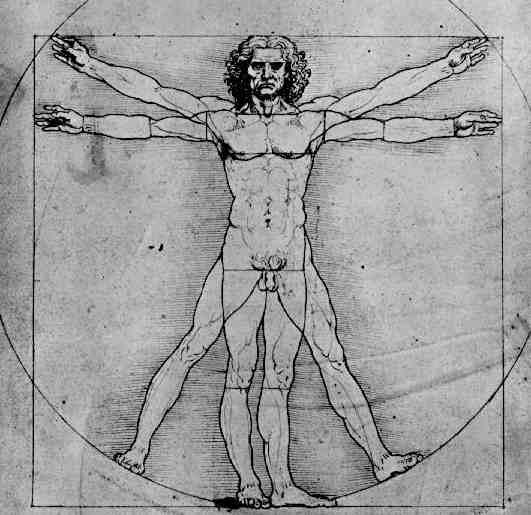
\includegraphics[height=50mm]{Figs/da-vinci-man.jpg}
\end{minipage}
\hspace{15mm}
\begin{minipage}[t]{50mm}
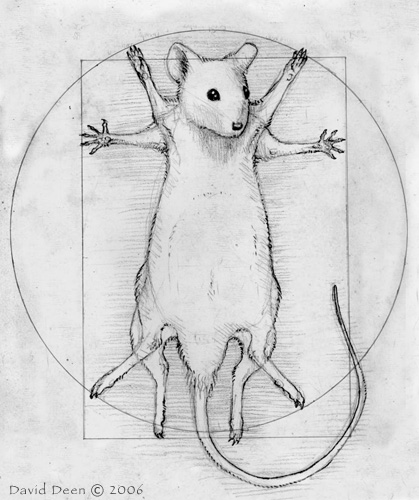
\includegraphics[height=50mm]{Figs/vitruvian_mouse.jpg}
\hspace{5mm}
\href{http://daviddeen.com}{\scriptsize \lolit \tt daviddeen.com}
\end{minipage}
}

\note{
   Of course, we're not really interested in curing mouse disease.
   Well, some of my collaborators are interested in mice specifically,
   but most studies of mice are carried out in order to learn about
   humans. And mice have a remarkable amount in common with humans.

   I like to think of mice as models for humans in three ways. First,
   the particular genes involved in a trait (say blood pressure) in
   the mouse could also be involved in the corresponding human trait.
   Second, the genetic architecture underlying a trait in the mouse
   (and the pathways and such) can tell us something about the genetic
   architecture of human traits. Finally, the methods we develop for
   gene mapping in mice might carry over to direct human studies.
}

\end{frame}





\begin{frame}[c]{Intercross}
\figw{Figs/intercross.pdf}{1.0}

\note{
  To learn about the genetics of a trait, we can perform one of a
  series of crosses; the most common is the intercross. You take two
  strains that differ in the trait of interest. Say the blue strain
  has low blood pressure and the pink strain has high blood pressure.
  You cross them and get the F$_1$ hybrid, which will get a copy of
  each chromosome. Then you cross F$_1$ siblings to get intercross
  progeny.

  The intercross mice will get a chromosome from each parent that
  could be the blue or pink chromosome intact but will more generally
  be a mosaic of the two chromosomes as a result of recombination at
  meiosis (the process of cell division that gives rise to sperm and
  egg cells).

  We would gather a bunch of intercross mice, measure the blood
  pressure of each (which could be the hardest part of this project),
  and then measure genotype along the chromosomes. We would then look
  for regions of the genome where genotype (whether a mouse was
  homoyzogous blue, heterozygous, or homozygous pink) is associated
  with the phenotype (blood pressure).

  Regions of the genome that affect a quantitative trait like blood
  pressure are called ``quantitative trait loci'' (QTL).
}

\end{frame}





\begin{frame}[c]{QTL mapping}

\vspace{5mm}
\figw{Figs/lodcurve_insulin_with_effects.pdf}{0.96}

\note{
  So we would then scan along the genome, at each position measuring
  the association between genotype and phenotype and plotting some
  test statistic.

  Effectively, we perform an ANOVA at each genomic position. (For
  historical reasons, we generally plot a different test statistic,
  the LOD score, which is a log$_{10}$ likelihood ratio comparing the
  hypothesis of genotype/phenotype association to the null hypothesis
  of no association.)

  Where the test statistic is large, there is some association between
  genotype and phenotype. So there will be a difference among the
  average trait values for the different genotypes, as seen here on
  chromosome 2, which is clearly not blood pressure (but rather, I
  think, log insulin level).
}

\end{frame}


\begin{frame}[c]{Congenic line}

\figw{Figs/congenic.pdf}{1.0}

\note{
  When we find a QTL, our goal is then to try to identify the gene
  underneath that location. The traditional approach is to form what's
  called a {\hilit congenic line}, where you take the blue strain and
  insert a chunk of the pink strain into it. If this new line shows a
  difference in phenotype from the blue strain, you have shown that
  something in that region is affecting the trait.

  You'd then do a series of crosses to break up that region into
  smaller and smaller pieces until you are able to pinpoint the
  particular gene that is responsible for the effect.

  This is very time consuming and expensive, and it is often not
  successful. QTL are usually mapped to very large intervals, like
  half a chromosome, and it takes a huge effort to fine map down to
  the gene level.

  So there's been a lot of effort to devise ways to speed up the process.
}

\end{frame}




\begin{frame}[c]{Advanced intercross lines}

  \figw{Figs/ail.pdf}{1.0}

\note{
  One approach is to do repeated generations of crosses to break up
  the chromosomes into smaller pieces. These are called advanced
  intercross lines. After 10 generations, you've broken up the
  chromosomes into much smaller pieces, and so the correlation among
  genotypes is much reduced and as a consequence your mapping
  precision is much higher.

  But this is really time consuming; you can only do about four
  generations of mice per year, so 10 generations is 2.5 years.
}

\end{frame}


\begin{frame}[c]{Recombinant inbred lines}

  \only<1>{\figw{Figs/rilines.pdf}{1.0}}
  \only<2|handout 0>{\figw{Figs/riself.pdf}{1.0}}

\note{
  Another approach is to create what are called recombinant inbred
  lines. You start with an intercross and then do repeated sibling
  mating to generate a new inbred line that has bits of each of the
  founder lines. Because of the multiple generations of crossing, you
  end up with more dense crossovers that occured in different
  generations. You do this multiple times in parallel to create a
  panel of lines that you can use for mapping.
  (Note that many plant species, you can do the same thing but using
  selfing rather than sib-mating: repeatedly crosses of a given plant
  to itself. The progress to inbreeding is much more rapid in that
  case.)

  This is also a lot of work, but the advantage here is that the final
  lines become a permanent resource. Once you've developed the lines,
  they can be shared among labs to study many different phenotypes.
  And you only need to genotype each line one time.
  There are a number of different panels of mouse RIL, but until
  recently they have been rather limited (like 10-15 lines from a
  given pair of founders). The BXD lines have been expanded
  considerably recently; there are like 80 or so BXD lines.

  But in addition to the disadvantage of the cost and time to develop
  such a panel, because they involve just two strains they are of
  interest only for traits that show a difference between those two
  particular founders. For example, the BXD panel may not be useful
  for your trait of interest.
}

\end{frame}


\begin{frame}[c]{Collaborative Cross}

  \figw{Figs/ri8.pdf}{1.0}


\note{
   In 2000, a group of mouse geneticists came up with the idea of the
   Collaborative Cross: to create a panel of recombinant inbred lines
   formed from a set of eight founders. The idea is you'd have the
   mapping resolution and other advantages of RILs, and since you were
   starting with a diverse set of lines, this single panel would be
   useful for a variety of purposes.
}

\end{frame}


\begin{frame}[c]{MAGIC}

  \figw{Figs/ri8self.pdf}{1.0}


\note{
  This idea has really taken off in plants, in which case they are
  called MAGIC lines. RILs by selfing from 8 or maybe even 16 or 32
  founders. There are MAGIC populations in Arabidopsis, wheat, maize,
  rice, and other plant species.
}

\end{frame}



\begin{frame}[c]{Heterogeneous stock}

  \vspace{2mm}

  \figh{Figs/hs.pdf}{0.9}


\note{
  The advanced intercross idea can also be extended to use more than
  two strains. An advanced intercross with 8 founders is sometimes
  called heterogeneous stock.
}

\end{frame}


\begin{frame}[c]{Collaborative Cross}

  \figw{Figs/ri8.pdf}{1.0}


\note{
  Back to these 8-way recombinant inbred lines, the Collaborative
  Cross: I became fascinated with the genotype pattern on the fixed,
  recombinant chromosome.
}

\end{frame}


\begin{frame}[c]{CC genome}

  \only<1>{\figw{Figs/ri8genome1.pdf}{1.0}}
  \only<2|handout:0>{\figw{Figs/ri8genome2.pdf}{1.0}}
  \only<3|handout:0>{\figw{Figs/ri8genome3.pdf}{1.0}}
  \only<4|handout:0>{\figw{Figs/ri8genome4.pdf}{1.0}}
  \only<5|handout:0>{\figw{Figs/ri8genome5.pdf}{1.0}}


\note{
  Here's a picture of a Collaborative Cross genome. At any one
  position, it's got one of the eight colors. What can we say about
  the rate of exchanges along the fixed chromosome, and are the
  switches equally likely among the eight colors? Can we calculate the
  transition matrix along the chromosome?
}

\end{frame}


\begin{frame}[c]{Recombination fraction}
  \figw{Figs/basic_genetics.pdf}{1.0}

\note{
  A key quantity to consider is the recombination fraction for an
  interval. If a parent has alleles A on one chromosome and B on the
  other, the sperm or egg cell produced at meiosis could have a
  parental type chromosomes, or it could have a so-called
  ``recombinant'' chromosome, with A at one locus and B at the other.
  The chance that meiosis produces a recombinant chromosome is called
  the recombination fraction. It depends on the distance between the
  two positions.

  Now the question is, for an interval that has recombination fraction
  $r$, what is the chance that the fixed Collaborative Cross
  chromosome will have the same allele, vs switch from one allele two
  another?  What's the analogous quantity to the recombination
  fraction for the fixed CC chromosome?
}

\end{frame}


\begin{frame}[c]{Simulation results}
  \figw{Figs/rf_by_sim.pdf}{1.0}

\note{
  I had this idea one night, and thought, ``I'll just simulate it.''
  So I started some simulations running: simulating the 8-way
  cross followed by repeated sibling mating until fixation, using
  intervals with different recombination fractions.

  The next morning I had this curve: the relationship between
  recombination fraction at meiosis (on the x-axis) and the chance
  that the CC chromosome is fixed for alternate alleles (on the
  y-axis). A nice smooth curve, and we can be confident that it hits
  7/8 when the recombination fraction is 1/2. (If the two positions
  are recombining completely at random, then you're picking two of the
  eight alleles for the two loci on the fixed chromosome, equally
  likely, and so there's a 7/8 chance that you'll pick different
  alleles.
}

\end{frame}


\begin{frame}[c]{Haldane \& Waddington 1931}

  \figw{Figs/haldane_title.pdf}{0.9}


\note{
  Well, I happened to know about this famous old paper that does this
  sort of calculation analytically for the two-way recombinant inbred
  line case. They cover sibling mating as well as selfing, and both
  autosomes and the X chromosome.
}

\end{frame}


\begin{frame}[c]{Result for selfing}

  \figw{Figs/haldane_selfing.png}{0.9}


\note{
   The paper is pretty hard going, but they derive some simple and now
   well-known equations, such as this one for selfing. If the
   recombination fraction (at meiosis) between two loci is $x$, then the
   chance the two-way RIL by selfing will be fixed for alternate
   alleles is $2x/(1+2x)$.
}

\end{frame}


\begin{frame}[c]{Result for sib-mating}

  \only<1>{\figw{Figs/haldane_sibmating3.png}{0.9}}
  \only<2>{\figw{Figs/haldane_sibmating4.png}{0.9}}


\note{
   For sib-mating, the result is $4x/(1+6x)$. That is, if the
   recombination fraction between two loci is $x$, the chance that
   two-way RIL by sibling mating will be fixed for alternate alleles
   is $4x/(1+6x)$.

   I particularly like that they say, ``Omitting some rather tedious
   algebra.'' If you've had a look at this paper, you may be surprised
   to then learn that there was tedious algebra {\hilit omitted}.
}

\end{frame}


\begin{frame}[c]{Simulation results}
  \figw{Figs/rf_by_sim_genformula.pdf}{1.0}

\note{
   So going back to my simulation results, I figured ``well, for
   2-ways by selfing it's $2x/(1+2x)$, and for 2-ways by sib-mating
   it's $4x/(1+6x)$, so maybe for 8-ways by sib-mating it's like $a x
   / (1 + b x)$ for some $a$ and $b$.
}

\end{frame}



\begin{frame}<handout:0>[fragile]{Non-linear regression}

\vspace{5mm}

{
\verb|    out <- nls(| {\tt \vhilit R \verb|~| a*r/(1 + b*r)}\verb|,| \\
\verb|               data = data.frame(r=r, R=R),| \\
\verb|               start = list(a=4, b=6))| \\
\verb|    summary(out)|
}


\end{frame}


\begin{frame}<handout:0>[fragile]{Non-linear regression}
\addtocounter{framenumber}{-1}

\vspace{5mm}

\verb|    out <- nls(| {\tt \vhilit R \verb|~| a*r/(1 + b*r)}\verb|,| \\
\verb|               data = data.frame(r=r, R=R),| \\
\verb|               start = list(a=4, b=6))| \\
\verb|    summary(out)|

\vspace{8mm}

{\hilit
\verb|                          | \\
\verb|      Estimate  Std. Error| \\
\verb|    a    7.016       0.011| \\
\verb|    b    6.023       0.016|
}


\end{frame}


\begin{frame}[fragile]{Non-linear regression}
\addtocounter{framenumber}{-1}

\vspace{5mm}

\verb|    out <- nls(| {\tt \vhilit R \verb|~| a*r/(1 + b*r)}\verb|,| \\
\verb|               data = data.frame(r=r, R=R),| \\
\verb|               start = list(a=4, b=6))| \\
\verb|    summary(out)|

\vspace{8mm}

{\hilit
\verb|                                       More data      | \\
\verb|      Estimate  Std. Error        Estimate  Std. Error| \\
\verb|    a    7.016       0.011      a    7.003       0.008| \\
\verb|    b    6.023       0.016      b    6.005       0.012|
}


\note{
  How can I figure out $a$ and $b$? Non-linear regression, using
  {\tt nls()} in R. It was immediately clear that the answer was
  $7r/(1+6r)$ for 8-way RIL by sib-mating. I did some more simulations
  to get more precise coefficient estimates, but the answer was clear.
}

\end{frame}


\begin{frame}[c]{Simulation results}
  \figw{Figs/rf_by_sim_moredata.pdf}{1.0}

\note{
   Add that curve to my simulated data and it fits perfectly. A
   triumph of computer simulation. Fancy algebra accomplished with no
   detailed knowledge whatsover. Certainly no tedious algebra.

   Okay, but not entirely satisfying. And by this point I was hooked:
   how to prove this equation?
}

\end{frame}


\begin{frame}[c]{Markov chain}

\bbi
\item Sequence of random variables $\mathsf{\{X_0, X_1, X_2, \dots\}}$
  satisfying

\vspace{2mm}

\centerline{\hilit $\mathsf{Pr(X_{n+1} \ | \ X_0,
X_1, \dots, X_n) = Pr(X_{n+1} \ | \ X_n)}$}

\item Transition probabilities {\hilit $\mathsf{P_{ij} =
  Pr(X_{n+1} = j \ | \ X_n = i)}$}

\item Here, $\mathsf{X_n}$ = ``parental type'' at generation n.

\item We are interested in {\vhilit absorption probabilities}

\vspace{2mm}

\centerline{\hilit $\pi_j = \mathsf{Pr(X_n \rightarrow j \ | \ X_0)}$}
\ei


\note{
  So they key thing here is that if you let $X_n$ denote the
  ``parental type'' meaning the pattern of alleles at two positions
  each of the two individuals' two chromosomes at generation $n$, then
  the $X$'s form a Markov chain. That is, if I tell you the pattern at
  a given generation, that's all you need to know to determine what
  will happen at the next generation; the history of how we got there
  doesn't matter.

  The key parameters for the Markov chain are the transition
  probabilities. That is, if I tell you the parental type at
  generation $n$, what are the probabilities for each possible type at
  generation $n+1$?

  The key thing we're trying to determine are so-called absorption
  probabilities. What is the chance that the Markov chain will be
  absorbed into a particular fixation state (from which it won't be
  able to exit), given the starting state (which is defined by the
  cross design).
}

\end{frame}



\begin{frame}[c]{Absorption probabilities}

  \bbi

  \item[] Consider the case of {\vhilit absorption} into the state
$\left.\begin{array}{c} \text{A} \\ \text{A} \end{array} \right| \begin{array}{c} \text{A}
  \\ \text{A} \end{array} $

\hspace*{15mm} {\hilit (write this $\mathsf{AA|AA}$)}

\item[] Let $\mathsf{h_i}$ = probability, starting at i, of being absorbed into $\mathsf{AA|AA}$.

\item[] Then {\hilit $\mathsf{h_{AA|AA}}$ = 1} and
{\hilit $\mathsf{h_{AB|AB}}$ = 0}.

\item[] {\vhilit Condition on the first step:} \hspace*{10mm}
{\hilit
%h$_{\text{i}}$ = $\sum_{\text{k}}$ P$_{\text{ik}}$ h$_{\text{k}}$}
$\mathsf{h_i  = \sum_k  P_{ik} h_k}$}

\item[] For selfing, this gives a system of 3 linear equations.
\ei


\note{
   A key trick with Markov chains is to condition on the first step.
   Let's focus on a particular absorbing state, say A's at both loci
   on both chromosomes. And let $h_i$ is the probability that,
   starting at state $i$, you'll be
   absorved into that particular $AA|AA$ state. Then $h_i$ is start at
   $i$, jump to state $k$, and from there be absorbed into the $AA|AA$
   state.

   So that gives us a set of linear equations that we can solve, since
   the transition matrix $P$ is known.

   For 2-way RIL by selfing, you end up with a system of three linear
   equations. There are five distinct states, but two are absorbing and
   so the $h$'s for them are just 0 or 1, so there are three unknowns.
}

\end{frame}



\begin{frame}[c]{Equations for selfing}

  \figw{Figs/haldane_selfing_equations.png}{0.9}


\note{
   Here's the 2-way selfing business from the Haldane and Waddington
   paper. They are showing the 5$\times$5 transition matrix and they
   go one to solve the set of related equations to get to that
   $2x/(1+2x)$ solution.
}


\end{frame}



\begin{frame}[c]{Equations for sib-mating}

  \figw{Figs/haldane_sibmating_equations.png}{0.9}


\note{
  The case of sibling mating is somewhat more complicated. There are
  22 distinct states to keep track of, and they're showing here the
  transition matrix.
}

\end{frame}


\begin{frame}[c]{Result for sib-mating}

  \figw{Figs/haldane_sibmating3.png}{0.9}

\note{
  Solving a system of equations that's a bit smaller but still rather
  similar to those, they get to the $4x/(1+6x)$ solution.

  Following this approach, I was able to prove my $7r/(1+6r)$
  equation, but by this time I had become obsessed with the situation
  for three points.
}

\end{frame}



\begin{frame}[c]{3-point coincidence}

\hfill \includegraphics[scale=0.5]{Figs/threepoints.pdf}

\vspace*{-15mm}

  \bbi

\item $\mathsf{r_{ij}}$ = recombination fraction for interval (i, j)

{\hilit Assume $\mathsf{r_{12} = r_{23} = r}$.}

\item {\vhilit Coincidence} = $\mathsf{c = Pr(\text{double
  recombinant}) / r^2}$

\hspace{20mm} {\hilit = $\mathsf{Pr(\text{rec'n in 23} \ | \ \text{rec'n in 12}) /
  Pr(\text{rec'n in 23})}$}

\item
No interference { \hilit = 1 }

Positive interference { \hilit $<$ 1 }

Negative interference { \hilit $>$ 1  }


\item Generally {\hilit $\mathsf{c}$} is a function of {\hilit $\mathsf{r}$}

  \ei



\note{
  I mentioned in the introductory lecture for this course about
  crossover interference: the tendency of these meiotic exchanges to
  not occur too close together. One measure of interference is to
  consider three points along a chromosome and calculate the so-called
  3-point coincidence, which you can view as the probability of
  exchange in both intervals divided by what would be expected by
  chance.

  Alternatively, and my preferred definition, is to think about
  recombination in the second interval, and ask how is the chance of a
  recombination event in the second interval affected by the presence
  of a recombination event in the first interval: the conditional
  probability divided by the prior probability.

  The coincidence being 1 indicates no interference, $<$ 1 indicates
  ``positive'' interference (crossovers tend not to be close
  together), and $>$ 1 indicates ``negative interference'' (crossovers
  tend to be clustered).

  The coincidence is generally a function of the size of the
  intervals, measured by the recombination fraction, $r$.
}

\end{frame}



\begin{frame}[c]{Coincidence}
\only<1|handout 0>{\figw{Figs/coincidence_ni.pdf}{1.0}}
\only<2>{\figw{Figs/coincidence_i.pdf}{1.0}}

\note{
  It turns out that, for 2-way recombinant inbred lines, the
  equivalent measure to coincidence for the fixed RIL chromosome can
  be derived directly with little effort, as it just depends on the
  recombination fraction for the three intervals (the two disjoint
  intervals plus the large interval that is the union of the two).
  The Haldane and Waddington paper has a section on this.

  The solid curves here are for the case of no crossover interference,
  with two-way RIL by selfing or sib-mating. In both cases, the curves
  are entirely above 1, indicating {\hilit clustering} of breakpoints
  on the fixed interval.

  Using a model for meiosis in the mouse, which exhibits strong
  positive crossover interference (the black dashed curve), we end up
  with the dashed curves for the coincidence-type quantity for the
  fixed chromosomes. For 2-way RILs by sib-mating, it is almost
  entirely above 1. This indicates that even if the crossovers at
  meiosis tend not to be close together, the breakpoints on the fixed
  RIL chromosome will tend to be clustered. Haldane and Waddington
  derived this, but didn't really dwell on it.
}

\end{frame}



\begin{frame}[c]{Coincidence in 8-way RILs}


\bbi
\item The trick that allowed us to get the coincidence for 2-way RILs
  doesn't work for 8-way RILs.

\item It's sufficient to consider 4-way RILs.

\item Calculations for 3 points in 4-way RILs is still {\vhilit
  astoundingly complex}.


\bi
\item {\hilit 2 points in 2-way RILs by sib mating:}

55 parental types $\rightarrow$ {\vhilit 22 states} by symmetry

\item {\hilit 3 points in 4-way RILs by sib mating:}

2,164,240 parental types $\rightarrow$ {\vhilit 137,488 states}
by symmetry
\ei

\item Even {\vhilit counting} the states was difficult.
\ei

\note{
  Now I'm interested in derived this quantity for 8-way RILs by
  sibling mating.  But it turned out that the trick used for 2-way
  RILs doesn't work for the 8-way case. However, it turns out it's
  sufficient to consider just 4-way RILs, because of the bottleneck
  with two parents each with two chromosomes.

  Still, it was difficult just to keep track of the possible states
  when 3 points on 4 chromosomes are considered.
}

\end{frame}



\begin{frame}[c]{Coincidence}
\figw{Figs/coincidence_8way.pdf}{1.0}

\note{
  Nevertheless, with some very hefty numerical calculations (not
  simulations, or algebra), I was able to derive the green equations
  here, which are the quantities analogous to the 3-point coincidence
  but for the fixed chromosome in 8-way RIL by sib-mating.

  Note that even with strong crossover interference, the coincidence
  is mostly above 1, again indicating clustering of breakpoints on the
  RIL chromosome. But really it's pretty close to 1, as for no
  interference.
}

\end{frame}




\begin{frame}[c]{The formula}

{ \fontsize{8.2pt}{9.2}\selectfont


$$ \mathsf{C = \frac{(1+6r)[280 + 1208r - 848r^2 + 5c(7-28r - 368r^2 + 344r^3)
  - 2c^2(49 - 324r + 452r^2)r^2 - 16c^3(1-2r)r^4]}{49 (1+12r-12cr^2)
    [5+10r-4(2+c)r^2+8cr^3]} }$$

}



\note{
  A few years later a collaborator showed me another trick to help in
  this work, and we were able to derive the exact formula for the
  3-point coincidence curve.
}

\end{frame}



\begin{frame}[c]{3-point symmetry}

\centerline{\hspace*{15mm} \hilit
$\mathsf{Pr(M_2 = x \ | \ M_1 = A, M_2 \ne A, M_3 = A)}$
}
\figw{Figs/3pt_symmetry.pdf}{1.0}


\note{
  There are some other interesting things you can look at here. First,
  concerning a sort of 3-point symmetry. If you observe A at the outer
  two of a set of three points and know that you had a double-exchange
  and were not A in the middle, what is the chance for each of the
  other seven alleles in the middle? In the cross
  A$\times$B$\times$C..., it turns out that you're unlikely to be B,
  because you'd need a double-crossover in that first meiosis, and
  you're more likely to be E,F,G, or H (which are all equally likely).
}

\end{frame}


\begin{frame}[c]{Markov property}

\centerline{\hspace*{15mm} \hilit
$ \mathsf{log_2 \left\{ \frac{Pr(M_3 = A \ | \ M_2 = A, M_1 = x)}{Pr(M_3 = A \ | \ M_2 = A)} \right\} }$
}
\figw{Figs/3pt_markov1.pdf}{1.0}


\note{
   You can also investigate the Markov property for the fixed 8-way
   RIL chromosome. If I tell you that you're A at point 2, how much
   does knowledge of point 1 tell you about the probabilities of what
   you end up being at point 3? Not very much in this case, with a
   non-exchange.
}

\end{frame}

\begin{frame}[c]{Markov property}

\centerline{\hspace*{15mm} \hilit
$ \mathsf{log_2 \left\{ \frac{
    Pr(M_3 = A \ | \ M_2 = {\vhilit B}, M_1 = x)}{
    Pr(M_3 = A \ | \ M_2 = {\vhilit B})}\right\}}$
}
\figw{Figs/3pt_markov2.pdf}{1.0}


\note{
   But how about if I ask about switching from B to A? Does knowledge
   of point 1 change your understanding of that? Well, if you were
   previously A and crossover interference is strong, you're very
   likely to {\hilit not} switch back to A, but otherwise it doesn't
   really matter.
}

\end{frame}



\begin{frame}[c]{Markov property}

\centerline{\hspace*{15mm} \hilit
$ \mathsf{log_2 \left\{ \frac{
    Pr(M_3 = A \ | \ M_2 = {\vhilit C}, M_1 = x)}{
    Pr(M_3 = A \ | \ M_2 = {\vhilit C})}\right\}}$
}
\figw{Figs/3pt_markov3.pdf}{1.0}


\note{
   But if I ask about switching from C to A, knowledge of the
   previous state can matter a lot. You're somehow more likely to
   switch from back to A from C, if you were previously A.
}

\end{frame}


\begin{frame}[c]{Markov property}

\centerline{\hspace*{15mm} \hilit
$ \mathsf{log_2 \left\{ \frac{
    Pr(M_3 = A \ | \ M_2 = {\vhilit E}, M_1 = x)}{
    Pr(M_3 = A \ | \ M_2 = {\vhilit E})}\right\}}$
}
\figw{Figs/3pt_markov4.pdf}{1.0}


\note{
  The same goes for the last case: switching from E to A is more
  likely if you'd previously been A. This is saying that you'll tend
  to have chunks of E stuck into the middle of a longer stretch of A.
  Which I did notice in simulations.
}

\end{frame}



\begin{frame}[c]{Whole genome simulations}

\bbi
\item 2-way selfing, 2-way sib-mating, 8-way sib-mating

\item Mouse-like genome, 1665 cM

\item Strong positive crossover interference

\item Inbreed to complex fixation

\item 10,000 simulation replicates
\ei


\note{
  I'd started out trying to sell you on the value of computer
  simulation, but now I've turned completely to numerical and then
  exact symbolic calculations. Simulations have the advantage of being
  easy to get started and get some quick solutions, but the results
  can be both imprecise (due to simulation error) and overly specific
  (due to difficulty of covering very general conditions).

  But let's get back to another way in which simulations have a big
  advantage over exact calculations: the ability to consider complete,
  realistic cases. In our exact calculations, we could look at two or
  three points along a chromosome. But there are a lot of interesting
  questions that can only be answered by considering the whole genome
  at once.

  So here we simulate recombinant inbred lines for a mouse-like genome
  with 20 chromosomes and a total genome length of 1665 cM.
}

  \end{frame}


\begin{frame}[c]{No. generations to fixation}
\figw{Figs/ngen_fix.pdf}{1.0}

\note{
  The first question: how many generations does it take to get
  complete inbreeding. We usually think of 6 generations for 2-way RIL by
  selfing and 20 generations for 2-way RIL by sibling mating, but here
  were seeing like 10 generations for selfing and 36 generations for
  sib-mating. 8-way RIL by sibmating take an extra 3 generations, but
  note that this includes the two extra generations to just get
  the 8 genomes together.
}

\end{frame}

\begin{frame}[c]{No. generations to 99\% fixation}
\figw{Figs/ngen99.pdf}{1.0}

\note{
  If we loosen the requirement of complete fixation and just look to
  see how long it takes to 99\% of the genome fixed, we cut off quite
  a bit, particularly from the sib-mating cases. But still note that
  while on average it takes 27 generations to get 99\% fixation in
  8-way RIL by sib-mating, there is a lot of variation; you could
  could be done in 20 or it could take 32 or so.
}

\end{frame}

\begin{frame}[c]{Percent genome not fixed}
\figw{Figs/prophet.pdf}{1.0}

\note{
   What percent of the genome is not fixed? Here we show the average
   and 95th percentiles be generation; impossible to get this
   analytically.
}

\end{frame}

\begin{frame}[c]{No. breakpoints}
\figw{Figs/nbrks.pdf}{1.0}

\note{
   How many crossovers are there, across the genome?
}

\end{frame}

\begin{frame}<handout:0>[c]{Segment lengths}
\figw{Figs/lseg_noarrows.pdf}{1.0}

\end{frame}

\begin{frame}[c]{Segment lengths}
\figw{Figs/lseg.pdf}{1.0}

\note{
   How big are the segments between crossovers? Note all of the spikes
   at whole chromosomes that were inherited intact.
}

\end{frame}

\begin{frame}[c]{Probability a segment is inherited intact}
\figw{Figs/probintact.pdf}{1.0}

\note{
  How likely is it that a particular segment is inherited intact, as a
  function of the length of the segment?
}

\end{frame}

\begin{frame}[c]{Length of smallest segment}
\figw{Figs/lsmseg.pdf}{1.0}

\note{
  What is the length of the smallest segment between crossovers,
  genome-wide?
}

\end{frame}

\begin{frame}[c]{No. segments $<$ 1 cM}
\figw{Figs/nsegsm1.pdf}{0.9}

\note{
  How many inter-breakpoint segments are $<$ 1 cM?
  An average of 11 in an 8-way RIL genome.

  Easy to answer by simulation; impossible to get at any other way.
}

\end{frame}



\begin{frame}[c]{Collaborative Cross}

  \figw{Figs/ri8.pdf}{1.0}


\note{
  Finish this work on the Collaborative Cross genomes, I'd thought I
  was done with this sort of applied probability. But then the
  first lines started to be developed, and they were wanting to
  genotype and phenotype them at intermediate generations, prior to
  full inbreeding. Which led to the question: what do these lines look
  like at the intermediate generations?
}

\end{frame}


\begin{frame}{The PreCC}


\vspace{5mm}

{\large What happens at $\mathsf{G_2 F_k}$?}

\bbi

\item[]  $\mathsf{Pr(g_1 = i)}$ \qquad\qquad {\hilit as a function of $\mathsf{k}$}

\item[]  $\mathsf{Pr(g_1 = i, g_2 = j)}$ \quad {\hilit as a function
      of $\mathsf{k}$ and the recombination fraction}
\ei


\note{
  We've covered the fully fixed chromosome case, but how about after
  $k$ generations of sibling mating? What are the genotype frequencies
  at a fixed point? What are the transition probabilities from one
  position to another?
}

\end{frame}


\begin{frame}[c]{Crazy table}
\figw{Figs/preCC_hap_prob_table.pdf}{1.0}

\note{
  So I was pulled back into this sort of investigation again, and
  while I wasn't able to solve all of the things I wanted, I was able
  to characterize the haplotype probabilities at these intermediate
  generations, which led to yet another rather crazy paper with this
  especially crazy table of results. ({\hilit Just try and re-type this table,
  copy editor; I dare you!})
}

\end{frame}


\begin{frame}[c]{Lesson}

  \centerline{\large Computer simulations are hugely valuable.}


\note{
  So I'd lost track of my the central theme several times in this, but
  the key lesson to draw from this is: computer simulations are hugely
  valuable for data scientists.
}

\end{frame}



\begin{frame}[c]{Uses of simulations}

    \bbi
    \item Study probabilities
    \item Estimate power/sample size
    \item Evaluate performance of a method
    \item Evaluate sensitivity/robustness of a method
    \ei


\note{
  Computer simulations have lots of uses: to study probabilities (as
  here), but also to estimate power or sample size, to evaluate how
  statistical methods perform, and to evaluate the sensitivity or
  robustness of a method.

  Are you're concerned about whether your method will work well if the
  data have errors or biases? Well, simulate data like you fear, and
  see try it out!
}

\end{frame}



\begin{frame}[c]{Relative advantages?}

    \bbi
    \item Simulations
    \item Numerical calculations
    \item Analytic calculations
    \ei


\note{
   In this work on recombinant inbred lines, I've used a combination
   of simulations, numerical calculations and analytic calculations.

   Analytic calculations can be the most satisfying, and can give you
   generally useful closed-form solutions. But you usually have to
   make a lot of simplifying assumptions, and it can be really hard
   work.

   Numerical calculations can have precision that approaches exact
   results, and can at times be easier to achieve and applicable in
   more complex cases.

   But computer simulations, while being potentially noisy and having
   to repeat everything for a variety of different cases, are often
   easy to get going and can allow consideration of fully realistic
   situations and to investigate complex outcomes.

   {\hilit When it doubt, simulate!}
}

\end{frame}




\begin{frame}[c]{References}

  \bbi

  \item Haldane \& Waddington (1931) Inbreeding and Linkage.
    Genetics 16:357--374

  \item Broman KW (2005) The genomes of recombinant inbred lines. Genetics 169:1133--1146

  \item Teuscher \& Broman (2007) Haplotype probabilities for
    multiple-strain recombinant inbred lines. Genetics 175:1267--1274

  \item Broman KW (2012) Genotype probabilities at intermediate
    generations in the construction of recombinant inbred lines.
    Genetics 190:403--412

  \item Broman KW (2012) Haplotype probabilities in advanced
    intercross populations. G3 2:199--202

  \ei


\note{
  Here are a bunch of references for the work I've presented.
}

\end{frame}

\end{document}
